\chapter{Numeryczne metody estymacji}

Przez \textbf{numerykę} rozumie się dziedzinę matematyki
zajmującą się rozwiązywaniem przybliżonych zagadnień algebraicznych. Odkąd zjawiska przyrodnicze zaczęto opisywać przy użyciu formalizmu matematycznego,
pojawiła się potrzeba rozwiązywania zadań analizy matematycznej czy algebry. Dopóki były
one nieskomplikowane, dawały się rozwiązywać analitycznie, tzn. z użyciem pewnych
przekształceń algebraicznych prowadzących do otrzymywania rozwiązań ścisłych danych
problemów. Z czasem jednak, przy powstawaniu coraz to bardziej skomplikowanych teorii
opisujących zjawiska, problemy te stawały się na tyle złożone, iż ich rozwiązywanie ścisłe
było albo bardzo czasochłonne albo też zgoła niemożliwe. Numeryka pozwalała znajdywać
przybliżone rozwiązania z żądaną dokładnością. Ich podstawową zaletą była ogólność tak
formułowanych algorytmów, tzn. w ramach danego zagadnienia nie miało znaczenia czy było
ono proste czy też bardzo skomplikowane (najwyżej wiązało się z większym nakładem pracy
obliczeniowej). Natomiast wadą była czasochłonność. Stąd prawdziwy renesans metod
numerycznych nastąpił wraz z powszechnym użyciem w pracy naukowej maszyn cyfrowych,
a w szczególności mikrokomputerów \cite{milewski}. Dziś dziesiątki żmudnych dla człowieka operacji
arytmetycznych wykonuje komputer, jednak złożoność obliczeniowa algorytmów uczących i modeli statystycznych stała się krytycznym czynnikiem ograniczającym w sytuacjach, gdy rozważane są duże zbiory danych. Te ograniczenia spowodowały, że w uczeniu maszynowym i modelowaniu statystycznym wielkiej skali zaczęto wykorzystywać algorytmy \textbf{stochastycznego spadku gradientu}. W poniższym rozdziale przedstawione są klasyczne algorytmy spadku wzdłuż gradientu Cauchy'ego oraz Raphsona-Newtona. Następnie omówiony jest algorytm stochastycznego spadku wzdłuż gradientu, którego wykorzystanie do estymacji współczynników w modelu Coxa jest kluczowym celem tej pracy. Algorytm stochastycznego spadku gradientu to metoda optymalizacji wzdłuż spadku gradientu wykorzystywana w sytuacjach, gdy rozważaną funkcję można zapisać jako sumę różniczkowalnych składników. Ponadto przedstawiono również zalety algorytmów stochastycznego spadku gradientu, które przemawiają za atrakcyjnością i popularnością tego typu rozwiązania. Ostatecznie przedyskutowano asymptotyczną efektywność estymatorów uzyskanych dzięki jednemu przejściu po zbiorze, zwanym \textit{epoką}. Definicje i pojęcia w tym rozdziale pochodzą z~\cite{bott1},~\cite{bott2},~\cite{kotlowski}~i~\cite{fortuna}.

\newpage
\section{Algorytmy spadku wzdłuż gradientu}\label{R-N}

Poniższy rozdział przedstawia popularne iteracyjne algorytmy wyznaczania przybliżonej wartości miejsca zerowego funkcji oraz rozważaną w pracy metodę stochastycznego spadku gradientu. Szukanie miejsc zerowych funkcji jest przydatne w problemach optymalizacyjnych, gdy celem jest znalezienie pierwiastka pochodnych badanej funkcji. Dodatkowo takie algorytmy wykorzystywane są do rozwiązywania (nieliniowych) układów równań. Metody iteracyjne składają się zazwyczaj z $k$ kroków bądź są zatrzymywane, gdy osiągnięty zostanie warunek stopu, czyli gdy odległość pomiędzy kolejnymi przybliżeniami jest dość mała $\parallel w_{k+1}-w_k\parallel < \epsilon$ lub wartość gradientu funkcji w wyznaczonym punkcie jest bliska wektorowymi zerowemu $\parallel \nabla_Q(\mathbf{w_k}) \parallel \leqslant \epsilon$ (test stacjonarności), gdzie $\epsilon$ to zadana z góry precyzja.
Metoda stochastycznego spadku wzdłuż gradientu zakłada, że minimalizowaną funkcję $Q(w)$ można przedstawić jako różniczkowalną sumę jej składników $Q(w) = \sum_{i=1}^{n}Q_i(w)$. W~poniższych algorytmach $\alpha_k$ oznacza długość kroku algorytmu.
\begin{center}
\textbf{Metoda spadku wzdłuż gradientu I (Cauchy’ego)}
\end{center}
Minimalizacja funkcji $Q(w)$:
\begin{itemize}
\item Zaczynamy od wybranego rozwiązania startowego, np. $w_{0} = 0$.
\item Dla $k = 1, 2, \dots$ aż do zbieżności
	\begin{itemize}
	\item Wyznaczamy gradient w punkcie $w_{k-1}, \nabla_{Q}(w_{k-1})$.
	\item Robimy krok wzdłuż negatywnego gradientu: $$w_{k} = w_{k-1} - \alpha_{k}\nabla_{Q}(w_{k-1}). $$
	\end{itemize}
\end{itemize}

\begin{center}
\textbf{Metoda spadku wzdłuż gradientu II (Newtona-Raphsona)}
\end{center}
Minimalizacja funkcji $Q(w)$:
\begin{itemize}
\item Zaczynamy od wybranego rozwiązania startowego, np. $w_{0} = 0$.
\item Dla $k = 1, 2, \dots$ aż do zbieżności
	\begin{itemize}
	\item Wyznaczamy gradient w punkcie $w_{k-1}, \nabla_{Q}(w_{k-1})$ i odwrotność Hesjanu $(D_{Q}^{2}(w_{k-1}))^{-1}$.
	\item Robimy krok wzdłuż negatywnego gradientu z zadanym krokiem przez Hesjan: $$w_{k} = w_{k-1} - (D_{Q}^{2}(w_{k-1}))^{-1}\nabla_{Q}(w_{k-1}). $$
	\end{itemize}
\end{itemize}
\begin{center}
\textbf{Metoda stochastycznego spadku wzdłuż gradientu I}
\end{center}
Minimalizacja funkcji $Q(w)$:
\begin{itemize}
\item Zaczynamy od wybranego rozwiązania startowego, np. $w_{0} = 0$.
\item Dla $k = 1, 2, \dots$ aż do zbieżności
	\begin{itemize}
	\item Wylosuj $i \in \{1,\dots,n\}$
	\item Wyznaczamy gradient funkcji $Q_{i}$ w punkcie $w_{k-1}, \nabla_{Q_{i}}(w_{k-1})$.
	\item Robimy krok wzdłuż negatywnego gradientu: 
	\begin{equation}\label{sgdrownanie}
	 w_{k} = w_{k-1} - \alpha_{k}\nabla_{Q_{i}}(w_{k-1}).
	  \end{equation}
	\end{itemize}
\end{itemize}

\section{Algorytm stochastycznego spadku wzdłuż gradientu I}\label{SGD}
Stochastyczny spadek gradientu to popularny algorytm wykorzystywany do estymacji współczynników w szerokiej gamie modeli uczenia maszynowego takich jak maszyny wektorów podpierających (\textit{ang. Support Vector Machines}), regresja logistyczna czy modele graficzne~\cite{finkel}. W~połączeniu z algorytmem propagacji wstecznej jest standardowym algorytmem w~trenowaniu sztucznych sieci neuronowych. Algorytm stochastycznego spadku gradientu był używany już od 1960 przy estymacji współczynników w modelu regresji liniowej, oryginalnie znanym jako \textit{ADALINE} \cite{ADALINE}. Kolejnym algorytmem wykorzystującym stochastyczny spadek gradientu jest filtr adaptacyjny najmniejszych średnich kwadratów \cite{widrow2} (\textit{ang.~least mean squares (LMS) adaptive filter}), który został wynaleziony przez Bernarda Widrowa, twórcę \textit{ADALINE}.

Idea algorytmu stochastycznego spadku gradientu jest następująca: zamiast obliczać gradient na całej funkcji $L$, w danym kroku oblicz
gradient tylko na pojedynczym elemencie $\ell_{i}$. Nazwa \textit{stochastyczny} bierze się stąd, iż oryginalnie wybiera
się element $\ell_{i}$ losowo. W praktyce zwykle przechodzi się po całym zbiorze danych w losowej kolejności.

\subsubsection{Właściwości stochastycznego spadku wzdłuż gradientu}

Zbieżność algorytmu stochastycznego spadku gradientu była szeroko badana w literaturze aproksymacji stochastycznych. Aby uzyskać zbieżność zazwyczaj wymaga się aby ciąg kroków algorytmu $\alpha_k$ był malejący i spełniał poniższe warunki $\sum\nolimits_k \alpha_k = \infty$ oraz $\sum\nolimits_k \alpha_k^2 < \infty$~\cite{bott1}.
Twierdzenie Robbinsa-Siegmunda \cite{robbins} przy łagodnych warunkach zapewnia~zbieżność~prawie na pewno \cite{bottDOD}, nawet  gdy~optymalizowana~funkcja~nie~jest~wszędzie~różniczkowalna.

Prędkość zbieżności stochastycznego spadku gradientu jest w rzeczywistości ograniczana przez zgrubną (\textit{ang. noisy}) aproksymacje prawdziwego gradientu. Gdy długości kroków algorytmu
maleją zbyt wolno, wariancja estymatorów parametrów $w_k$ maleje równie wolno. Gdy kroki algorytmu maleją
zbyt szybko, oczekiwane estymatory parametrów $w_k$ potrzebują więcej czasu by osiągnąć optimum \cite{bott1}. Pod pewnymi warunkami regularności \cite{murata}, najlepsza prędkość zbieżności jest uzyskana dla kroków algorytmu $\alpha_k\sim k^{-1}$.

Jak wykazano w \cite{dennis} pod pewnymi odpowiednimi warunkami regularności, gdy zainicjowany współczynnik początkowy $w_0$ jest wystarczająco blisko optimum i krok algorytmu jest odpowiednio mały, algorytm stochastycznego spadku gradientu osiąga liniową zbieżność. Oznacza to, iż przy spełnieniu założeń metody, odległości pomiędzy kolejnymi przybliżeniami a minimum funkcji $\mathbf{w^{\ast}}$ maleją liniowo: $\parallel \mathbf{w^{\ast}} - \mathbf{w_{k+1}} \parallel \leqslant c \parallel \mathbf{w^{\ast}} - \mathbf{w_k} \parallel$. Zbieżność wymaga często przejścia parokrotnie po całym
zbiorze danych. Wady i zalety algorytmu wymienione są poniżej. Zalety~zdecydowanie przewyższają~wady.

\textbf{Zalety} \vspace{-5pt}
\begin{itemize}
\item \textcolor{orange}{Szybkość}: obliczenie gradientu wymaga wzięcia tylko jednej
obserwacji.
\item \textcolor{orange}{Skalowalność}: cały zbiór danych nie musi nawet znajdować się
w pamięci operacyjnej.
\item \textcolor{orange}{Prostota}: gradient funkcji  $Q_{i}$ daje bardzo prosty wzór na
modyfikacje wag.
\end{itemize}

\textbf{Wady}  \vspace{-5pt}
\begin{itemize}
\item \textcolor{orange}{Wolna zbieżność}: czasem gradient stochastyczny zbiega wolno
i wymaga wielu iteracji po zbiorze uczącym.
\item \textcolor{orange}{Problem z ustaleniem długości kroku $k$}: wyznaczenie $k$
przez przeszukiwanie liniowe nie przynosi dobrych rezultatów,
ponieważ nie optymalizujemy oryginalnej funkcji $Q$ tylko jej jeden
składnik $Q_{i}$.
\end{itemize}
\newpage
\section{Porównanie algorytmów spadku wzdłuż gradientu}

W niniejszym podrozdziale przedstawiono graficznie różnice w wyborze kolejnych punktów w trakcie optymalizacji między omawianymi w poprzedniej części pracy algorytmami spadku wzdłuż gradientu I (Cauchy'ego), spadku wzdłuż gradientu II (Newtona-Raphsona) oraz stochastycznego spadku wzdłuż gradientu I. W celu zobrazowania przykładu na dwuwymiarowym wykresie, postanowiono ograniczyć się do modelu z jedną zmienną objaśniającą i wyrazem wolnym. Do przykładu wybrano model regresji logistycznej, z racji na prostotę przedstawienia funkcji log-wiarogodności jako sumy różniczkowalnych składników.

Funkcja log-wiarogodności dla modelu regresji logistycznej, za \cite{czepiel} i \cite{dobson}, ma postać

\begin{equation}
\marginnote{$\beta=(\beta_1,\beta_2)$}
\ell(\beta) = \sum\limits_{i=1}^{N}\Big(y_i(\beta_1+\beta_2x_i) -\log(1+\exp(\beta_1+\beta_2x_i))\Big) = \sum\limits_{i=1}^{N} Q_i(\beta_1,\beta_2), 
\end{equation}
\begin{equation}
Q_i(\beta_1,\beta_2) = y_i(\beta_1+\beta_2x_i) -\log(1+\exp(\beta_1+\beta_2x_i)).
\end{equation}

Dla tak skonstruowanej funkcji wiarogodności, współrzędne gradientu to odpowiednio

\begin{equation*}
\dfrac{\partial\ell(\beta)}{\partial\beta_1} = \sum\limits_{i=1}^{N}\Big(y_i-\pi_i(\beta)\Big), \ \ \ \ \
\dfrac{\partial\ell(\beta)}{\partial\beta_2} = \sum\limits_{i=1}^{N}x_i\Big(y_i-\pi_i(\beta)\Big),
\end{equation*}

zaś macierz informacji wyraża się jak następuje
\begin{equation}\label{iii}
\mathscr{I}(\beta) = 
\begin{bmatrix}
    \sum\limits_{i=1}^{N}\pi_i(\beta)(1-\pi_i(\beta))       & \sum\limits_{i=1}^{N}x_i\pi_i(\beta)(1-\pi_i(\beta)) \\
\sum\limits_{i=1}^{N}x_i\pi_i(\beta)(1-\pi_i(\beta)) & \sum\limits_{i=1}^{N}x_i^2\pi_i(\beta)(1-\pi_i(\beta)) 
\end{bmatrix},
\end{equation}
gdzie $\pi_i(\beta) = \frac{\exp(\beta_1+\beta_2x_i)}{1+\exp(\beta_1+\beta_2x_i)}$, a $N$ to liczba obserwacji.

Wtedy aktualizacja kandydata na miejsce zerowe w $k$-tym kroku algorytmu optymalizacyjnego dla kolejnych metod omówionych w rozdziale (\ref{R-N}) wyraża się poniższymi wzorami
\\
\begin{center}
\textbf{Metoda spadku wzdłuż gradientu I (Cauchy’ego)}
\end{center}
\begin{equation*}
\beta_{k} = \beta_{k-1} + \alpha_{k}\cdot\Big(\sum\limits_{i=1}^{N}(y_i-\pi_i(\beta_{k-1})), \sum\limits_{i=1}^{N}x_i(y_i-\pi_i(\beta_{k-1}))\Big).\marginnote{$\alpha_k \in \mathbb{R}$}
\end{equation*}
\begin{center}
\textbf{Metoda spadku wzdłuż gradientu II (Newtona-Raphsona)}
\end{center}
\begin{equation*}
\beta_{k} = \beta_{k-1} + \mathscr{I}(\beta_{k-1})^{-1}\cdot\Big(\sum\limits_{i=1}^{N}(y_i-\pi_i(\beta_{k-1})), \sum\limits_{i=1}^{N}x_i(y_i-\pi_i(\beta_{k-1}))\Big),
\end{equation*}
gdzie $\mathscr{I}(\beta_{k-1})$ zdefiniowane jest we wzorze (\ref{iii}). 
\begin{center}
\textbf{Metoda stochastycznego spadku wzdłuż gradientu I}
\end{center}
\begin{equation*}
\beta_{k} = \beta_{k-1} + \alpha_{k}\cdot\Big(y_i-\pi_i(\beta_{k-1}), x_i(y_i-\pi_i(\beta_{k-1}))\Big),
\end{equation*}
dla wylosowanego w danym kroku $i$.
\\ \ \\
Ponieważ algorytmy te znajdują minimum funkcji, a docelowo szukane jest maksimum, stąd wykorzystano przeciwieństwo funkcji log-wiarogodności, dlatego w wyżej wymienionych wzorach zmieniono znaki przed pochodnymi na przeciwne.

\newpage
Poniższymi wywołaniami kodów z pakietu $\mathcal{R}$ \cite{programikr} można otrzymać wartości ekstremum w danym kroku kolejnych algorytmów. Kod funkcji \texttt{logitGD()} oraz fragmenty kodu tworzące poniższy wykres dostępne są w Dodatku~\ref{kody}.
\begin{Shaded}
\begin{Highlighting}[]
\NormalTok{x <-}\StringTok{ }\KeywordTok{rnorm}\NormalTok{(}\DecValTok{1000}\NormalTok{)}
\NormalTok{z <-}\StringTok{ }\DecValTok{2} \NormalTok{+}\StringTok{ }\DecValTok{3}\NormalTok{*x}
\NormalTok{pr <-}\StringTok{ }\DecValTok{1}\NormalTok{/(}\DecValTok{1}\NormalTok{+}\KeywordTok{exp}\NormalTok{(-z))}
\NormalTok{y <-}\StringTok{ }\KeywordTok{rbinom}\NormalTok{(}\DecValTok{1000}\NormalTok{,}\DecValTok{1}\NormalTok{,pr)}

\KeywordTok{logitGD}\NormalTok{(y, x, }\DataTypeTok{optim.method =} \StringTok{"GDI"}\NormalTok{, }\DataTypeTok{eps =} \FloatTok{10e-5}\NormalTok{, }\DataTypeTok{max.iter =} \DecValTok{500}\NormalTok{)$steps ->}\StringTok{ }\NormalTok{GDI}
\KeywordTok{logitGD}\NormalTok{(y, x, }\DataTypeTok{optim.method =} \StringTok{"GDII"}\NormalTok{, }\DataTypeTok{eps =} \FloatTok{10e-5}\NormalTok{, }\DataTypeTok{max.iter =} \DecValTok{500}\NormalTok{)$steps ->}\StringTok{ }\NormalTok{GDII}

\NormalTok{ind <-}\StringTok{ }\KeywordTok{sample}\NormalTok{(}\KeywordTok{length}\NormalTok{(y))}
\KeywordTok{logitGD}\NormalTok{(y[ind], x[ind], }\DataTypeTok{optim.method =} \StringTok{"SGDI"}\NormalTok{,}
        \DataTypeTok{max.iter =} \DecValTok{500}\NormalTok{, }\DataTypeTok{eps =} \FloatTok{10e-5}\NormalTok{)$steps ->}\StringTok{ }\NormalTok{SGDI}\FloatTok{.1}
\end{Highlighting}
\end{Shaded}


\begin{figure}[h]
  %\vspace{-10pt}
  %\begin{center}
   \subfigure[Symulacja 1.]{
     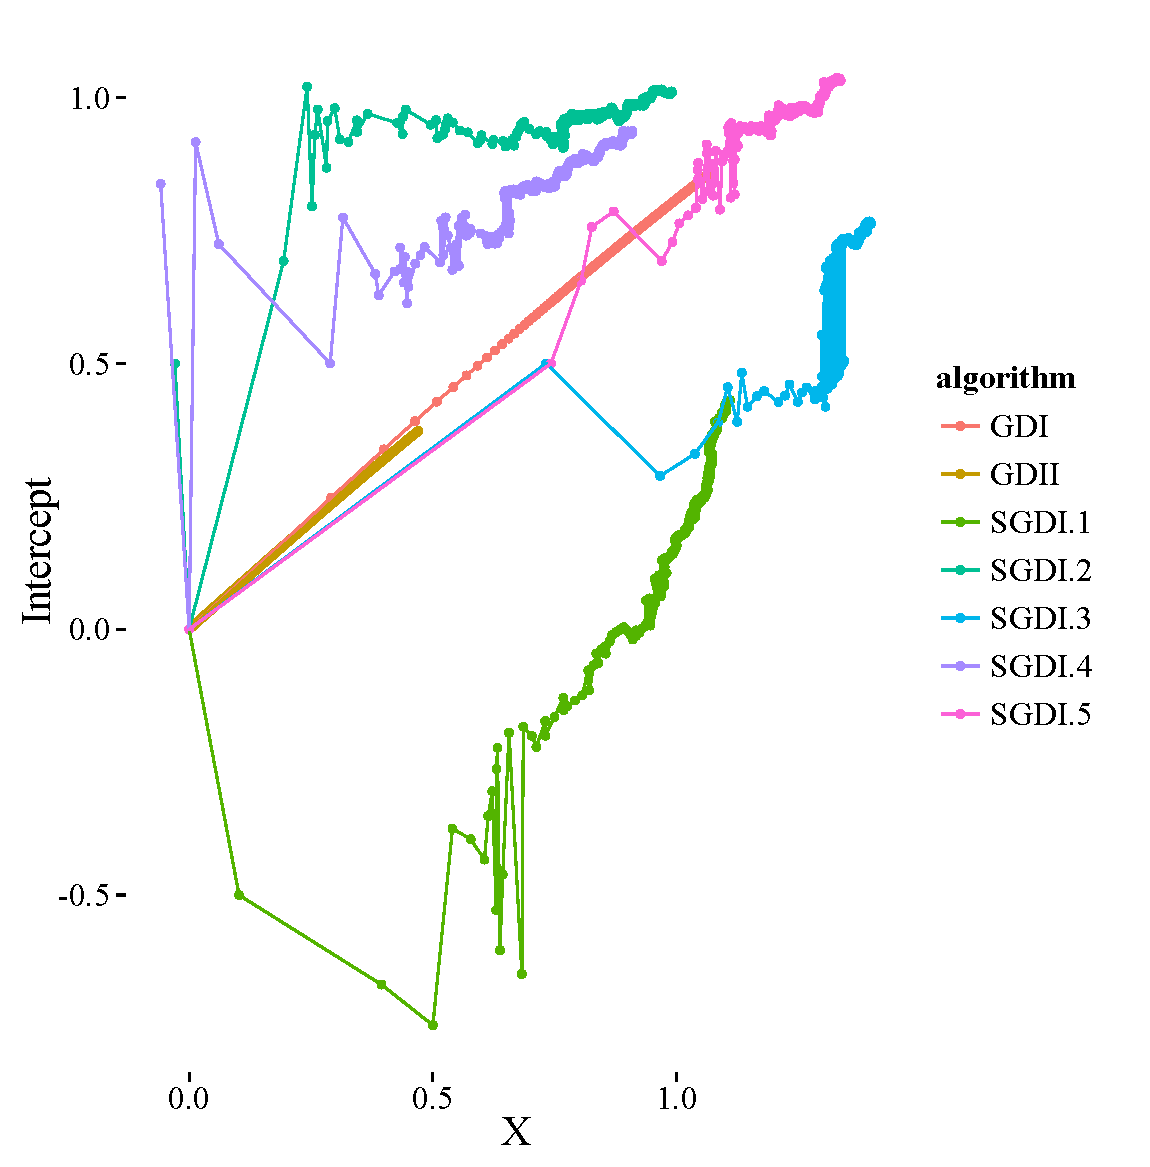
\includegraphics[width=0.32\textwidth]{Obrazki/Rplot.pdf}}
   \subfigure[Symulacja 2.]{
     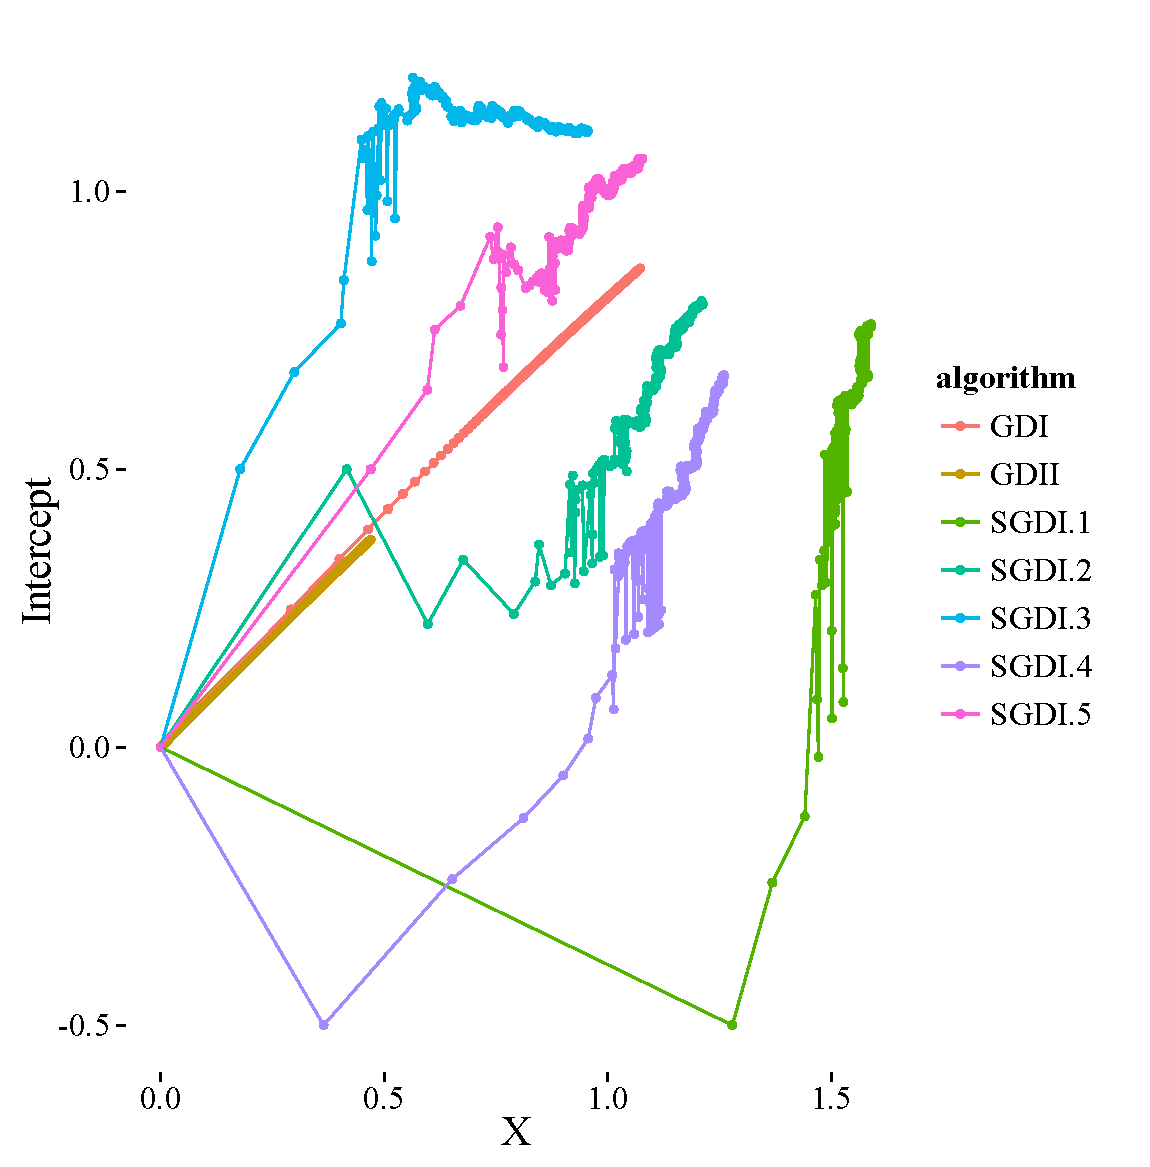
\includegraphics[width=0.32\textwidth]{Obrazki/Rplot02.pdf}}
   \subfigure[Symulacja 3.]{
     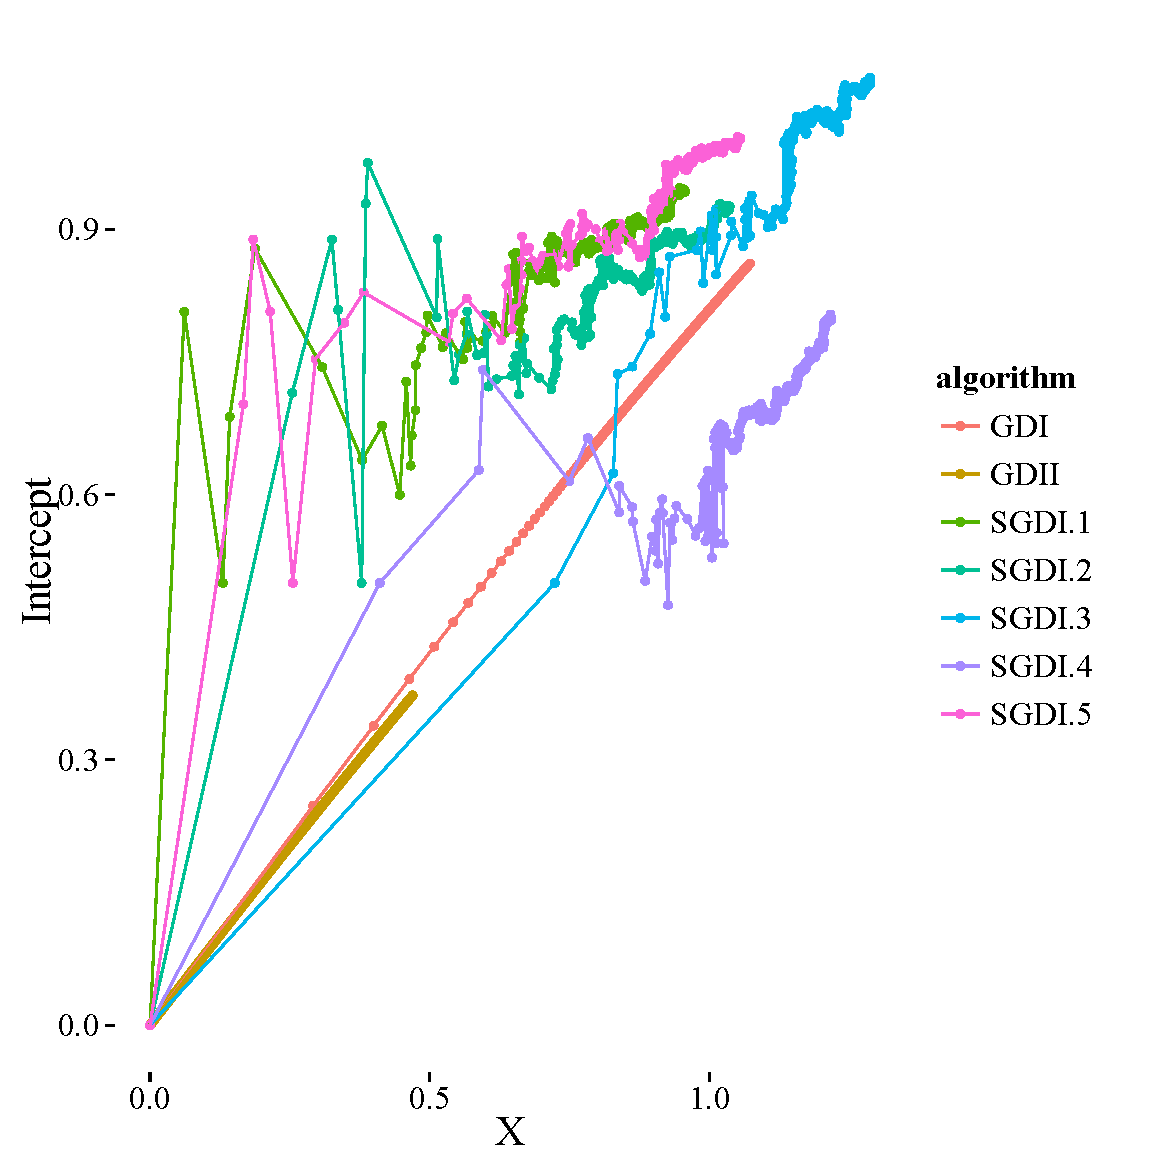
\includegraphics[width=0.32\textwidth]{Obrazki/Rplot03.pdf}}
   \subfigure[Symulacja 4.]{
     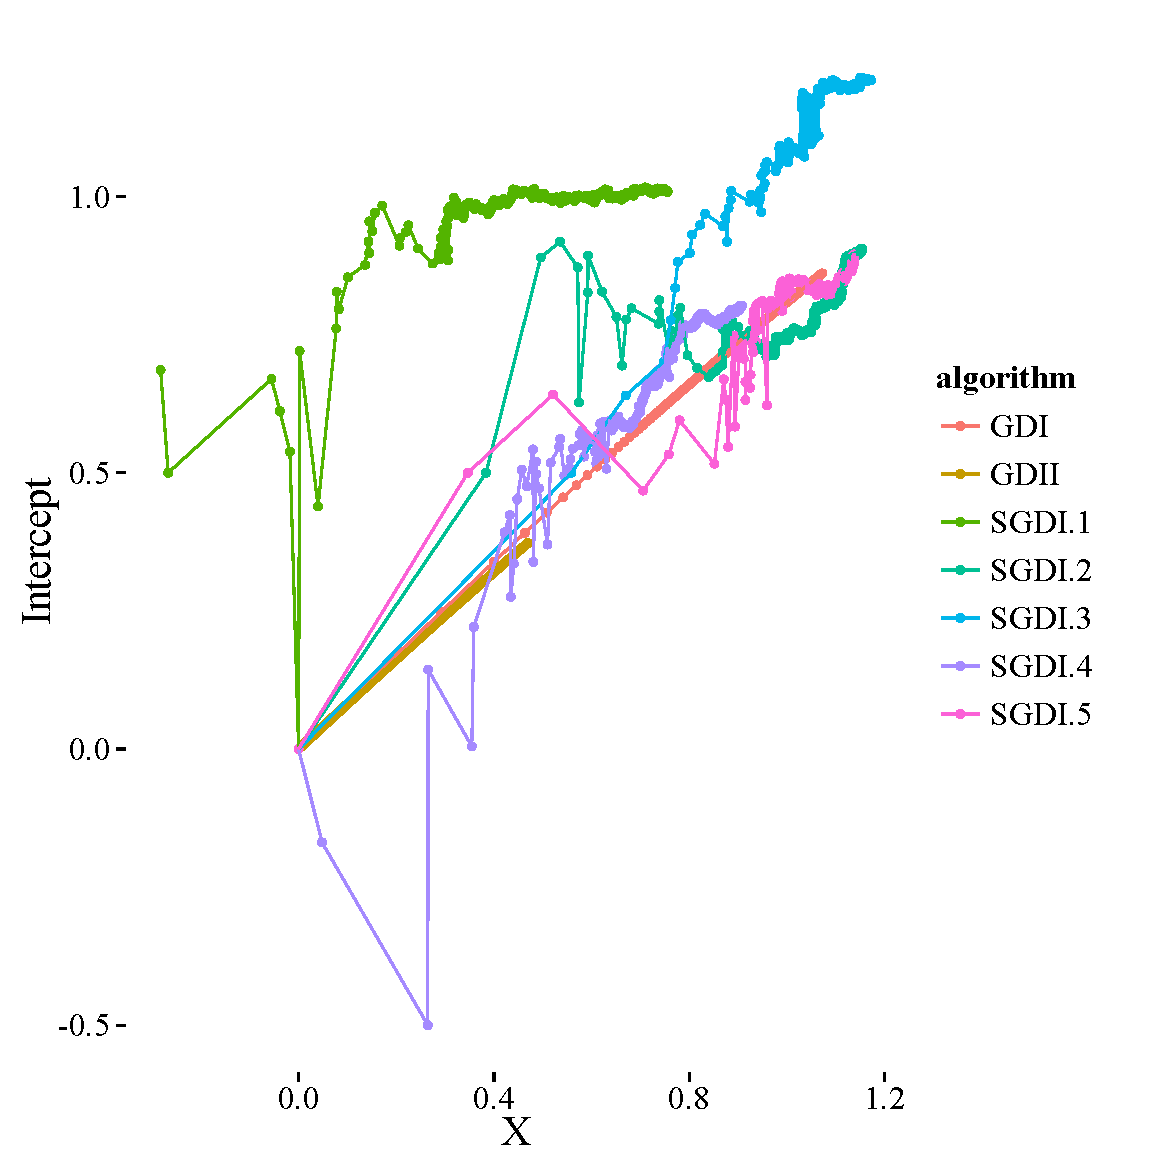
\includegraphics[width=0.32\textwidth]{Obrazki/Rplot04.pdf}}
   \subfigure[Symulacja 5.]{
     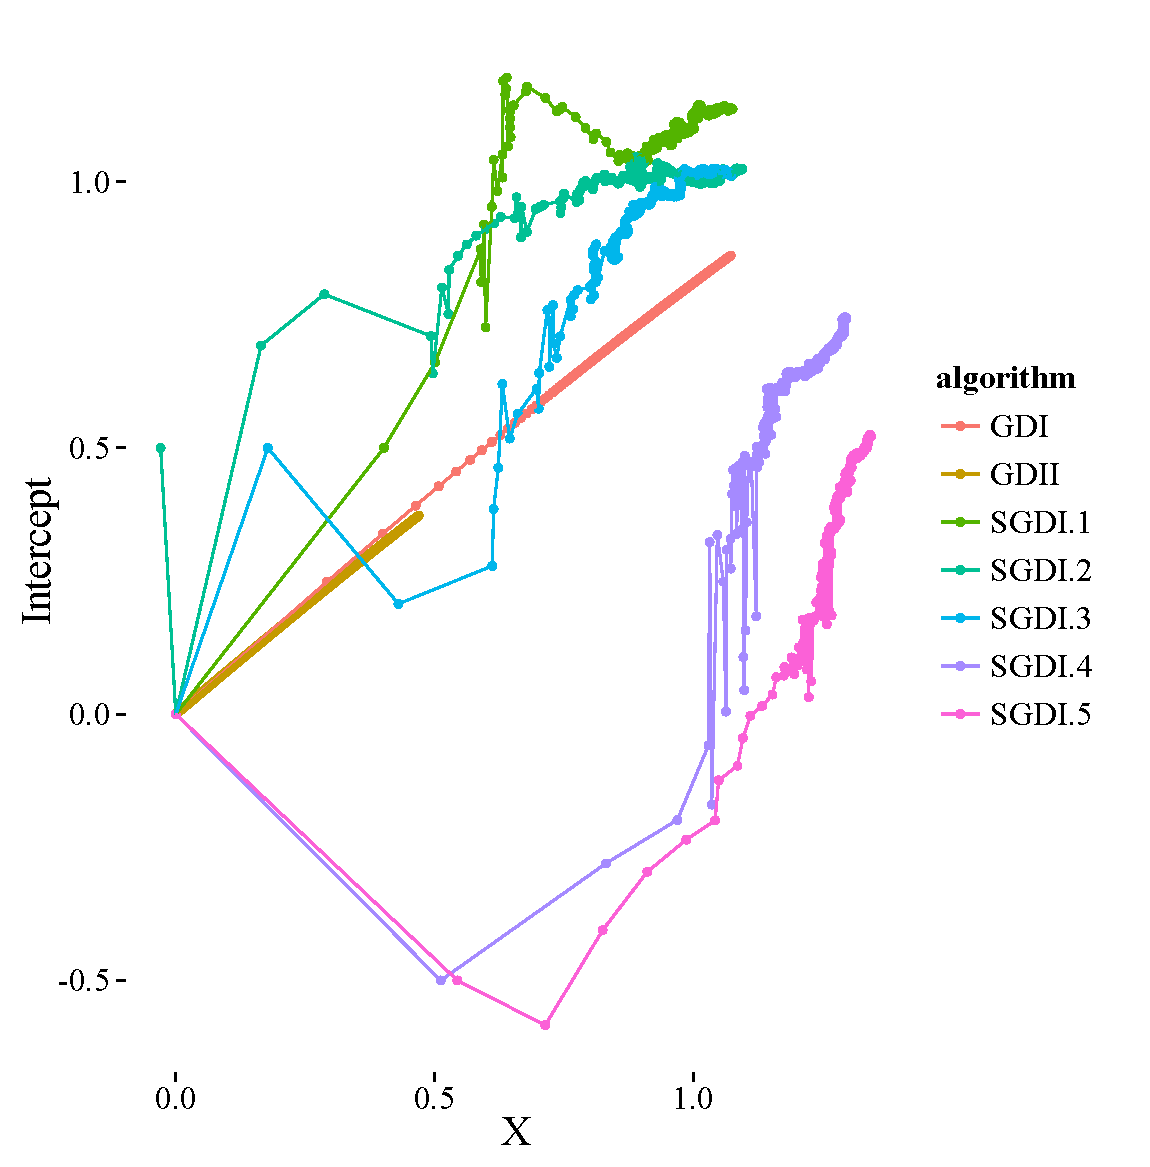
\includegraphics[width=0.32\textwidth]{Obrazki/Rplot05.pdf}}
   \subfigure[Symulacja 6.]{
     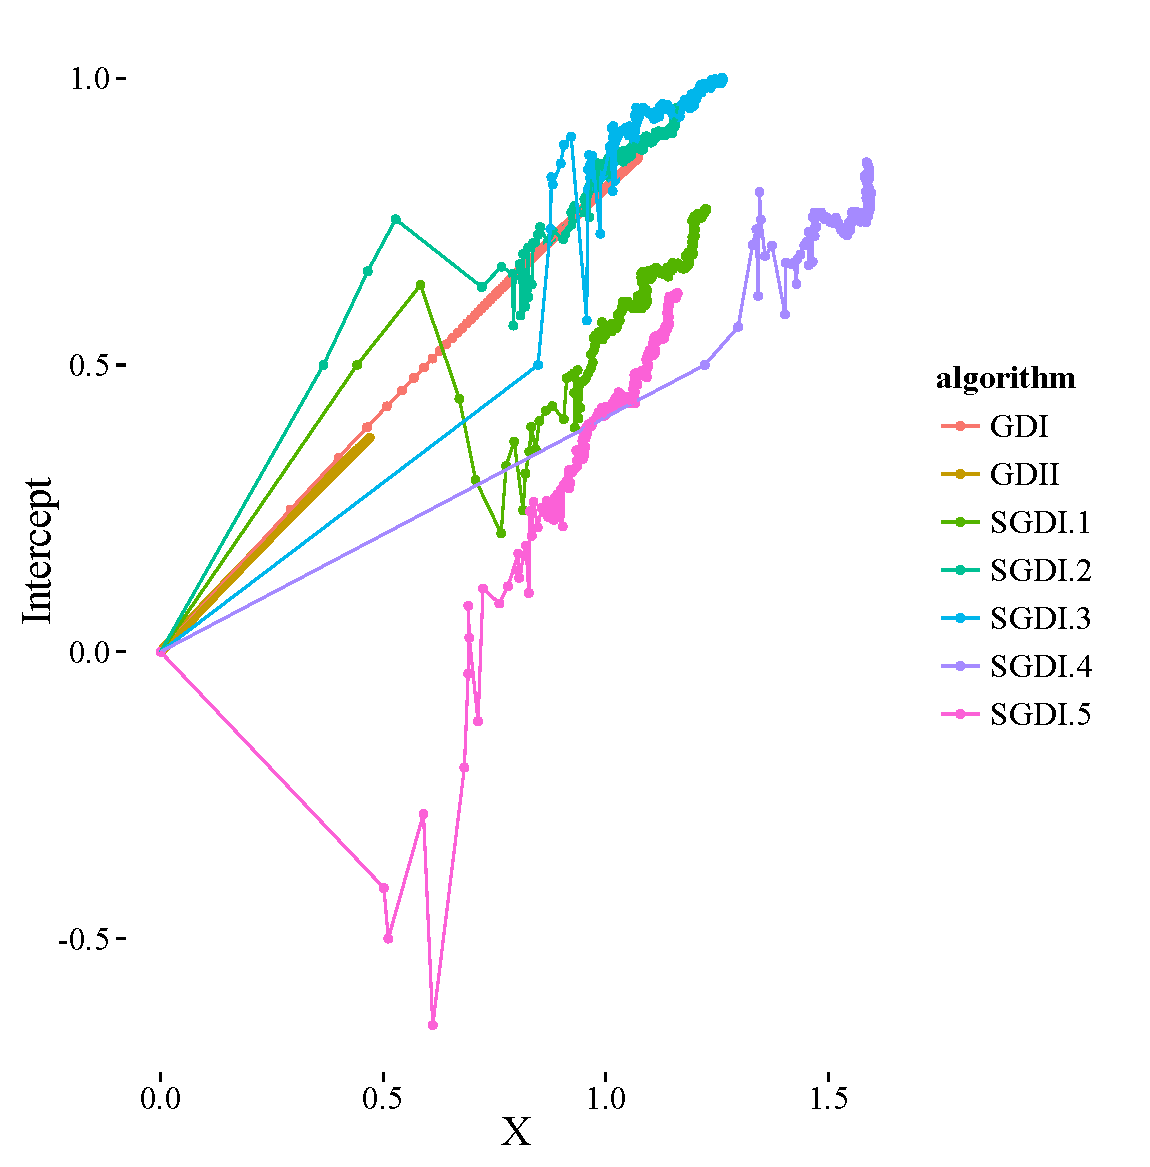
\includegraphics[width=0.32\textwidth]{Obrazki/Rplot06.pdf}}
  %\end{center}
  %\vspace{-10pt}
  \label{fig:sc}
  \caption{Porównanie algorytmów spadku gradientu.}
\end{figure}

Powyższe wywołania zostały wykonane 6 razy i przedstawione na 6 oddzielnych wykresach. Na każdym wykresie pięciokrotnie naniesiono kolejne kroki optymalizacji algorytmem stochastycznego spadku gradientu. Widać, że stochastyczna istota algorytmu powoduje, że za każdym razem trajektoria zbiegania do optimum podczas minimalizacji jest inna jednak kierunek ostatecznie w dużej mierze pokrywa się algorytmami niestochastycznymi.
